\documentclass[12pt]{article}
\usepackage{amsmath}
\usepackage{mathrsfs}
\usepackage{graphicx}
\usepackage{wrapfig}
\usepackage{booktabs}
\usepackage[letterpaper, margin=1in]{geometry}
\usepackage{fancyhdr}
\usepackage [autostyle, english = american]{csquotes}
\MakeOuterQuote{"}
\renewcommand{\baselinestretch}{1.0}
\newcommand{\objects}[2]{%
  \leavevmode\vbox{\hbox{#1}\nointerlineskip\hbox{#2}}%
}
\title{Lab 5 \\ Analysis of Sequential Circuits}
\author{Qadis Chaudhry}
\date{April 23, 2021}
\begin{document}
\maketitle
    \section*{Experiment 1}
    \begin{figure}[h]
        \centering
        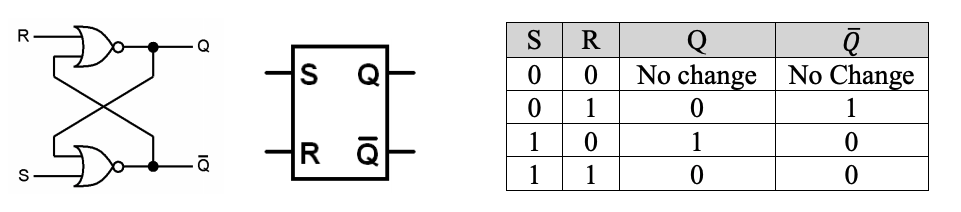
\includegraphics[width=0.9\textwidth]{SRLatch.png}
        \caption{The SR-latch}
    \end{figure}
    \par Given above is the design of the SR-latch as well as its function
    summarized within a table. The SR-latch takes in two inputs, $S$ and $R$,
    and outputs two values, $Q$ and $\overline{Q}$, where $\overline{Q}$ is the
    compliment of $Q$. This latch is designed with the intent of storing the
    value of $Q$ and it does this based on the combination of $S$ and $R$.  The
    function is achieved with the use of two NOR gates where one of the inputs
    to the gate is one of the outputs coupled with either $S$ or $R$. By doing
    this, the value of $Q$ depends on the combination of $R$ and $S$ as well as
    the previous state of $Q$, for example, when the value of $S$ is 0 and $R$
    is 1, the value of $Q$ will be set to zero.
    \par The table above is a more general summary of the function since it does
    not include the current state of the output $Q$, however, it is an accurate
    representation of the function of the device since the examination of the
    circuit realizes that no matter the current value of $Q$, whenever the
    combination of $S R = 01$, the output value of $Q$ will be 0.  Similarly,
    when $S R = 01$, the value of $Q$ will always result as 1. This is the basic
    function of the SR-latch and the way it achieves such function. There is one
    state however in which this device breaks down and that is when $S R = 11$.
    Here, the value of $Q$ as well as $\overline{Q}$ will be 0 and this is known
    as the "forbidden" state since the values of $Q$ and $\overline{Q}$ are the
    same.  Since $\overline{Q}$ is the compliment of $Q$, this behavior is not
    appropriate and therefore invalidates the device at this input combination.
    \par Now, this circuit can be implemented using the Verilog HDL in one of
    two ways, traditionally defining the individual gates and their inputs, or
    with the use of behavioral programming. The first method seems to be the
    most straight forward, defining both NOR gates as well as their inputs and
    outputs and the circuit is finished from there. However, another means of
    implementing this circuit is with behavioral programming, programming where
    the user defines a certain set of expectations of the circuit and Verilog
    will create a circuit based on those expectations. For this implementation,
    behavioral programming will be employed.
    \begin{figure}[h]
        \centering
        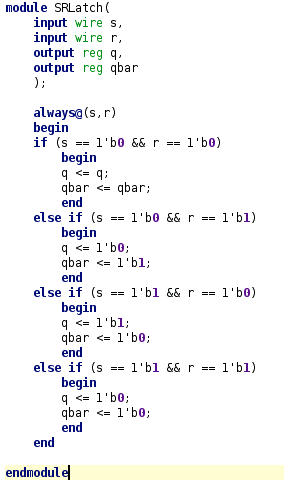
\includegraphics[width=0.3\textwidth]{SRLatch Code.png}
        \caption{SR-latch Code}
    \end{figure}
    \par This is the code for the SR-latch within Verilog using the concept of
    behavioral programming. It can be seen that there are  no specifically
    defined gates within the code rather, the code consists of parameters
    defining what the output should be based on the inputs. At the top there are
    the inputs to the module, $s$ and $r$, and the outputs, $q$ and $qbar$, and
    after that is where the behavioral programming is specified. It starts with
    the declaration of the condition under which the proceeding statements are
    run, \textit{always@(s,r)}. This block is began with the \textit{begin}
    statement and will end with the corresponding \textit{end} statement, and
    implies that the statements written within this block will be executed with
    the values of $s$ and $r$.
    \par Next, a collection of \textit{if} statements can be seen and these are
    responsible for the specification of the conditions under which the outputs
    should be changed. The first statement runs when the values of $s$ and $r$
    are 00 respectively. Next comes the \textit{begin} statement to initiate the
    start of the block, and within this block it can be seen that the variable
    $q$ is set to $q$, and the variable $qbar$ is set to $qbar$. This defines
    the first row of the table that described the SR-latch, when $S R = 00$,
    there results in no change to the values of $Q$ and $\overline{Q}$. This is
    known as the \textit{hold} state of the latch as it "holds" the previous
    value of $Q$. The next statement is another conditional statement,
    \textit{else if}, and this executes when the \textit{if} statement before it
    turns out to be false. In this case, this will happen when the value of $s
    r$ is not $00$, and the condition given to this block is when $s r = 01$. If
    this is true, the values of $q$ and $qbar$ will be set to 0 and 1
    respectively. The next two conditional statements do the same, in accordance
    with the table and the result should be a circuit that provides the function
    of the SR-latch.
    \begin{figure}[h]
        \centering
        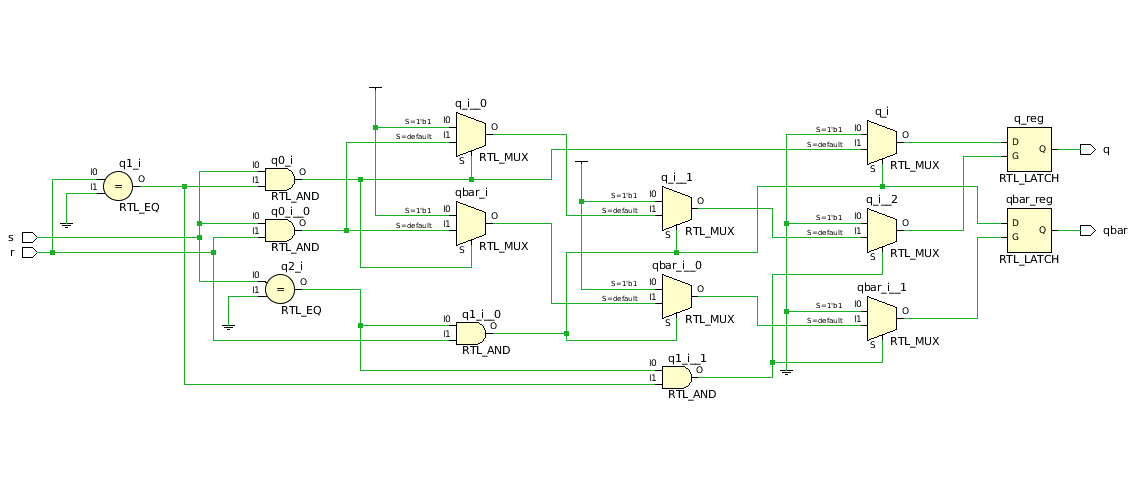
\includegraphics[width=1.0\textwidth]{SRLatch Schematic.png}
        \caption{SR-latch Schematic}
    \end{figure}
    \par Above is the generated schematic based on the written code and it can
    be seen that the circuit generated is far more complicated than expected.
    This is due to the fact that Verilog does not resort to using the fewest
    number of gates to achieve the functionality specified instead, it looks
    solely to meet the expectations of the circuit. In this case, that meant
    that the program was not looking for the output to be connected back into
    the input of two NOR gates rather, it was to use all the gates available to
    it in order to achieve the functionality. The only way that we can ensure
    that this provides the correct function, is through the examination of the
    waveform that is generated by this circuit. Once that is done, it will be
    clear whether this circuit is correct or not.
    \begin{figure}[h]
        \centering
        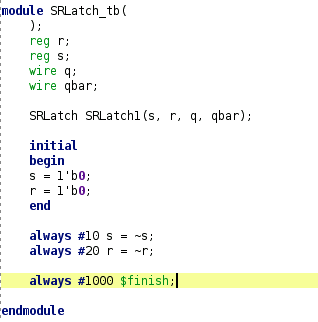
\includegraphics[width=0.4\textwidth]{SRLatch Simulation Code.png}
        \caption{SR-latch Simulation Code}
    \end{figure}
    \par This is the set up of the simulation for the generated circuit. At the
    top, the inputs are initialized using the keywords, \textit{reg} and
    \textit{wire}, and then the latch module is instantiated. The module for the
    latch was named "SRLatch," and here it can be seen that it is being
    implemented for the production of the waveform. After this, the input values
    are initialized as $s r = 00$. This gives the program a starting point and
    next we can see how the values of the inputs change, how this is reflected
    within the outputs and in the waveform as well. Once again, with the
    \textit{always} keyword, the simulation is told to oscillate the values of
    $s$ and $r$ between 0 and 1. This is done simply by setting the values to
    their compliment after a set period of time, in this case, every 10
    nanoseconds for $s$ and every 20 nanoseconds for $r$. Lastly, the simulation
    is given an termination time of 1,000 nanoseconds. With this, the simulation
    is set up and the generated waveform is ready to be analyzed to see whether
    or not the created circuit provides the function of an SR-latch.
    \begin{figure}[h]
        \centering
        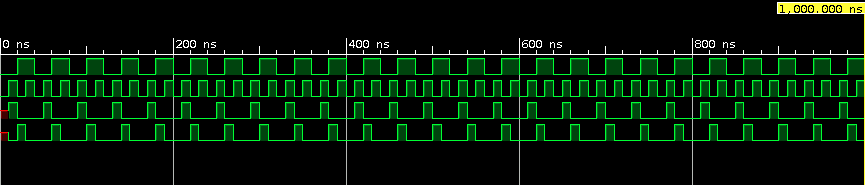
\includegraphics[width=1.0\textwidth]{SRLatch Waveform.png}
        \caption{SR-latch Waveform}
    \end{figure}
    \par The execution of the simulation generates the above waveform. The
    output values $q$ and $qbar$ are shown as the two waves on the bottom, and
    the input values $r$ and $s$, shown as the first two waves from the top.
    The timings for the changes in the variables allow for all possible
    combination of $S$ and $R$ can be covered, 00, 01, 10, and 11, this way, all
    the possible outputs are depicted. With the analysis of the waves, it can be
    seen that the values generated at the output are in accordance with the
    table for the latch, when $s$ and $r$ are both 1, the value of $q$ equals 0,
    when both values are 0, the value of $q$ remains constant, and the set and
    reset states are present in accordance to the table as well. This explicates
    that despite its complicated appearance, the circuit generated by the
    program is a functional SR-latch.
    \newpage
    \subsection*{NOR Gate Implementation of SR-latch}
    \begin{figure}[h]
        \centering
        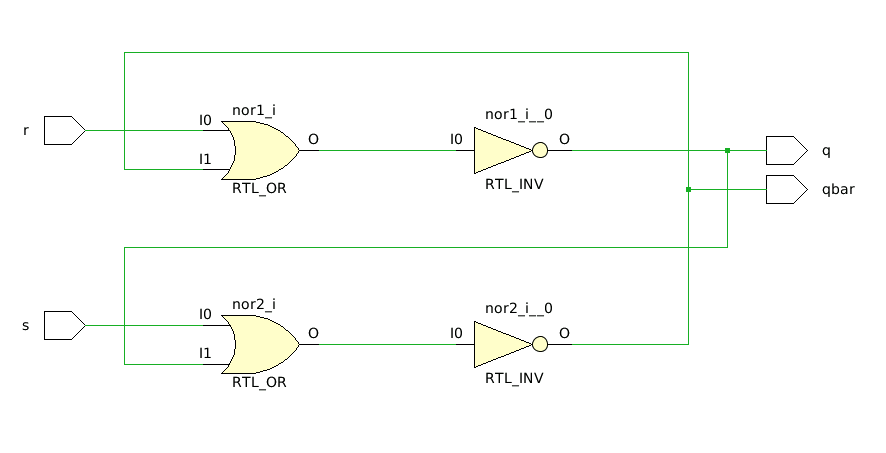
\includegraphics[width=0.7\textwidth]{NOR Gate SRLatch.png}
        \caption{NOR Gate SR-latch}
    \end{figure}
    \par As stated before, instead of using behavioral programming to implement
    this latch, the traditional method of defining gates and their inputs and
    outputs can be used. From the schematic above, it can be seen that this
    circuit is much more in line with the one shown in the design of the
    SR-latch, there are two NOR gates where the inputs of the gates are $s$ and
    $q$, and $r$ and $qbar$.
    \begin{figure}[h]
        \centering
        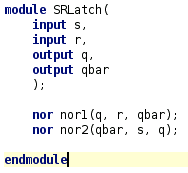
\includegraphics[width=0.3\textwidth]{NOR Gate SRLatch Code.png}
        \caption{NOR Gate SR-latch Code}
    \end{figure}
    \par This is the code for the implementation of this circuit and it can be
    seen that it is far simpler than the previous implementation. Instead of
    using conditional statements and expressing logical behaviors, this
    implementation makes use of the built in NOR gate to create the circuit.
    The inputs are specified at the top as $s$ and $r$, as well as the outputs,
    $q$ and $qbar$. The only thing that this implementation requires is that the
    two NOR gates are specified with their inputs and outputs. The top NOR gate
    can be seen taking the inputs $r$ and $qbar$ and outputting $q$, while the
    bottom NOR gate takes in the inputs $s$ and $q$ and outputs $qbar$. This is
    an exact replica of the design circuit and it will be seen with the waveform
    that both implementations of the latch are identical.
    \newpage
    \begin{figure}[h]
        \centering
        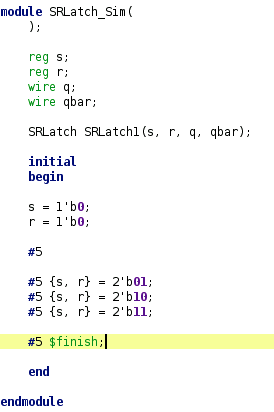
\includegraphics[width=0.3\textwidth]{NOR Gate SRLatch Simulation Code.png}
        \caption{NOR Gate SR-latch Simulation Code}
    \end{figure}
    \par This is the code for the simulation of the NOR gate implementation of
    the SR-latch in Verilog. In this case, the inputs and outputs are manually
    given values instead of having them be changed autonomously after a given
    time period. At the top, the inputs and outputs are initialized and the
    latch module, still named "SRLatch," is instantiated with the inputs $s$ and
    $r$, and the outputs $q$ and $qbar$. Next, the simulation is began and the
    input values are set to 00. After 5 nanoseconds, the simulation begins to
    change, $s r$ is given a value of $01$, then again after 5 nanoseconds, the
    value is changed to 10, and then once again changed to 11, and then finally
    after the last 5 nanoseconds the simulation is terminated. In this case, all
    of the changes were manually specified and the simulation was ended at the
    end of these changes as well which means that this simulation will last a
    total of 25 nanoseconds.
    \begin{figure}[h]
        \centering
        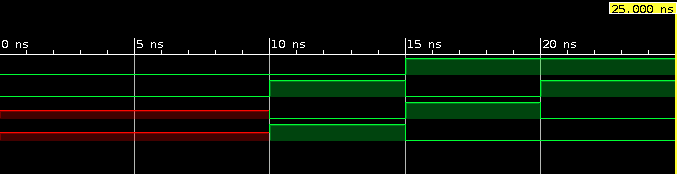
\includegraphics[width=1.0\textwidth]{NOR Gate SRLatch Waveform.png}
        \caption{NOR Gate SR-latch Waveform}
    \end{figure}
    \par Here, it can be seen that the outputs change on the changes of the
    input and for the first 10 nanoseconds, there is no activity in the
    waveform. This is because for an SR-latch, when the values of $s$ and $r$
    both equal 0, the latch is in the hold state. Since there were no values
    initially defined for $q$ and $qbar$, the values here are marked as don't
    cares. With the changes to the values of $S$ and $R$ however, it can be seen
    that the values of $Q$ and $\overline{Q}$ change respectively, $S R = 01 \to
    Q \overline{Q} = 01$, $S R = 10 \to Q \overline{Q} = 10$, $S R = 11 \to Q
    \overline{Q} = 00$. In accordance with the table for the SR-latch, the
    circuit provides the functionality of the SR-latch.
    \section*{Experiment 2}
    \begin{figure}[h]
        \centering
        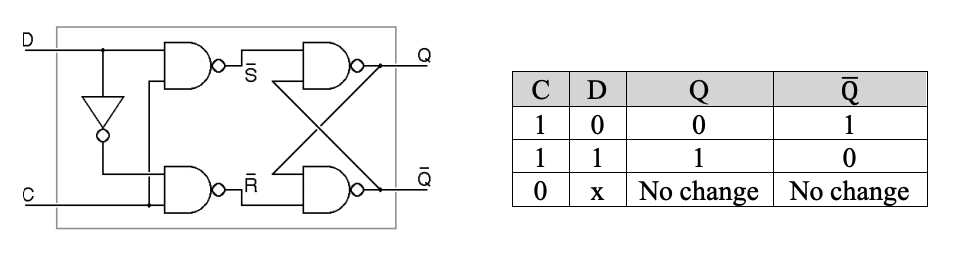
\includegraphics[width=0.8\textwidth]{DLatch.png}
        \caption{The D-latch}
    \end{figure}
    \par This is the design for the D-latch and it can be seen that it is
    similar to the SR-latch in that, it has the same cross connection from the
    output to the input. The D-latch stems straight from the concept of the
    SR-latch and from the table it can be seen that it provides similar function
    as well, however, the main difference is that there is no "forbidden" state
    with this latch. Made up of two NAND gates as well as one main input, $D$,
    the D-latch can provide useful functionality by controlling the output $Q$
    with very little changes in the input. Since there are only two inputs, $D$
    and a control $C$, there are simply three possible states that $Q$ can
    manifest. When $C$ equals 0, the output is controlled and $Q$ harbors no
    change, and when $C$ is equal to 1, the output $Q$ will follow whatever the
    value of $D$ is, either 0 or 1. Since there is only really one input, there
    is no possibility for $Q$ and $\overline{Q}$ to be the same value. This
    means that this latch is valid for all the possibilities of the input,
    unlike the SR-latch. This latch can be implemented using Verilog as well and
    the code is simpler than that of the SR-latch.
    \begin{figure}[h]
        \centering
        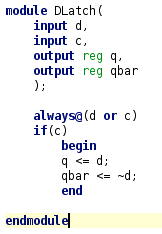
\includegraphics[width=0.25\textwidth]{DLatch Code.png}
        \caption{D-latch Code}
    \end{figure}
    \par This is the code for the implementation of a D-latch within Verilog and
    it simply consists of one conditional statement. The inputs and outputs are
    initialized as the arguments of the module and given as, inputs $d$ and $c$,
    and outputs $q$ and $qbar$. The \textit{if} statement checks the value of
    $c$ since in the case that $c = 0$, the latch does nothing and the value of
    $q$ remains unchanged. On the other hand, if the value of $c$ equals 1, the
    statement executes and the value of $q$ as set to the present value of $d$
    and $qbar$ is set to the compliment of $d$.
    \begin{figure}[h]
        \centering
        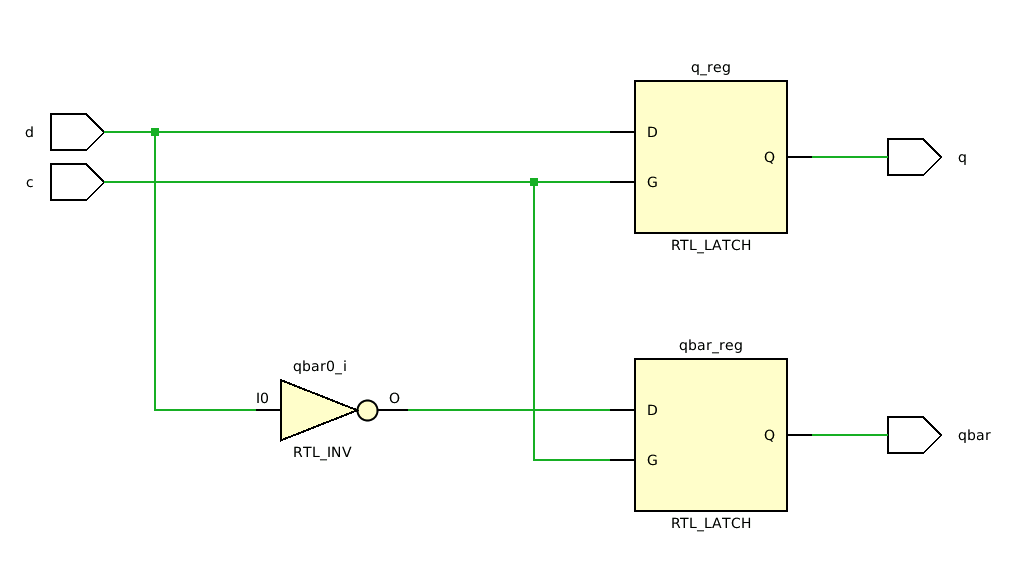
\includegraphics[width=0.6\textwidth]{DLatch Schematic.png}
        \caption{D-latch Schematic}
    \end{figure}
    \par Once again, the circuit generated seems to look esoteric as it uses
    multiple gates which are not expected. In this case, as previously, the
    analysis of the waveform will lead to the conclusion of whether or not this
    circuit provides the functionality of the D-latch.
    \begin{figure}[h]
        \centering
        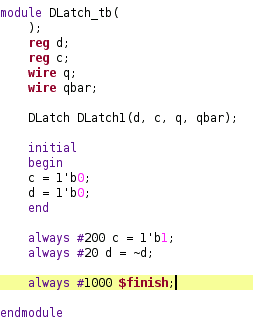
\includegraphics[width=0.3\textwidth]{DLatch Simulation Code.png}
        \caption{D-latch Simulation Code}
    \end{figure}
    \par This code is for the simulation of the D-latch circuit and it is
    similar to that of the SR-latch however, this time there is really only one
    input that needs to be monitored and the other is set to change at a
    specific time in the simulation to see its effect in the waveform. The
    "DLatch" module is instantiated and given the inputs $d$ and $c$, and the
    outputs $q$ and $qbar$. The \textit{initial} keyword beings the simulation
    and the values of the inputs are set to 00. At 200 nanoseconds, the value of
    $c$ is changed from 0 to 1 and every 20 nanoseconds the value of $d$ is
    changed to its compliment. The simulation is given a termination time of
    1,000 nanoseconds and with that, is ready to be run.
    \begin{figure}[h]
        \centering
        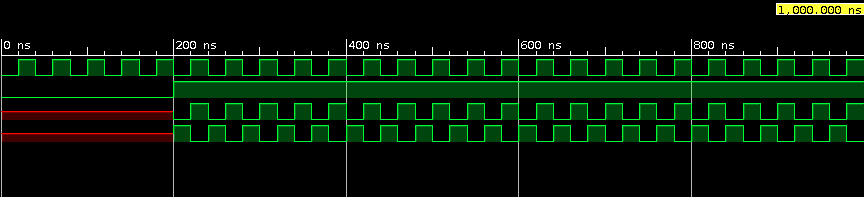
\includegraphics[width=1.0\textwidth]{DLatch Waveform.png}
        \caption{D-latch Waveform}
    \end{figure}
    \par This is the waveform generated by the circuit for the coded D-latch.
    The inputs are shown as the first two waves, $d$ and $c$ respectively, and
    the outputs $q$ and $qbar$ are shown as the bottom two waves. At 200
    nanoseconds, the value of $c$ goes from 0 to 1 and it can be seen that prior
    to this transition, the values of $q$ and $qbar$ were given by don't cares.
    This is because the value of $q$ and $qbar$ do not change when $c=0$, and
    since no initial value of the outputs was specified, they are labeled as
    don't cares as their values are unknown and don't change. Moving past that,
    when the value of $c$ equals 1, it can be seen that the value of $q$ follows
    the value of $d$, and the value of $qbar$ is the compliment. This is exactly
    the expected behavior of the D-latch and from this, it can be deduced that
    the circuit generated, as well as the code written for it, provides the
    proper functionality of the D-latch.
    \section*{Experiment 3}
    \begin{figure}[h]
        \centering
        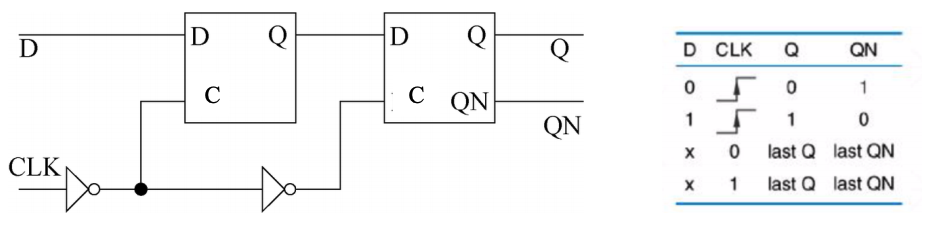
\includegraphics[width=0.8\textwidth]{DFlipFlop.png}
        \caption{The D-Flip-Flop}
    \end{figure}
    \par Shown above is the design of the D-flip-flop and its function
    summarized in a table. A flip-flop is another form of a state machine and is
    distinguished from a latch by the fact that it requires a clock for its
    operation. The particular flip-flop is called the D-flip-flop as it is
    formed by coupling two D-latches and a clock. The clock's main purpose is
    for the genesis of the change within the circuit. This design shown above is
    a positive edge triggered D-flip-flop which means that the changes in the
    output will only occur at the positive edge cycle of the clock. The same
    functionality as the D-latch is observed, $Q$ will follow the value of $d$,
    however, while the clock is in its other phases the last value of $Q$ and
    $\overline{Q}$ will be held. This circuit can be very easily implemented
    with Verilog as well since the only difference here is the inclusion of the
    clock.
    \begin{figure}[h]
        \centering
        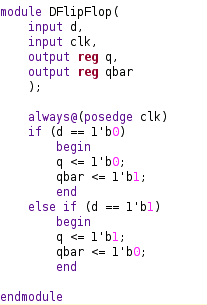
\includegraphics[width=0.3\textwidth]{DFlipFlop Code.png}
        \caption{D-Flip-Flop Code}
    \end{figure}
    \par This is the code for the D-flip-flop and it is quite close to that of
    the D-latch, the main difference being that the outputs are set to change at
    the positive edge of the clock rather than with the change of the inputs.
    The module begins with the definition of the inputs and outputs and here, it
    can be seen that instead of the input $c$, there is an input $clk$.  The
    clock replaces the control input since it is now the clock the relays the
    output changes. Next, the \textit{always@(posedge clk)} declares that the
    proceeding statements must only execute at the positive edge of the clock
    cycle. After this come the conditional statements and this time the values
    for the input $d$ are being directly evaluated. In the case that $d$ equals
    0, the output $q$ follow the input and will also equal 0. The same is true
    for $d=1$, the output $q$ will equal 1 as well. The schematic for this
    circuit can now be generated.
    \begin{figure}[h]
        \centering
        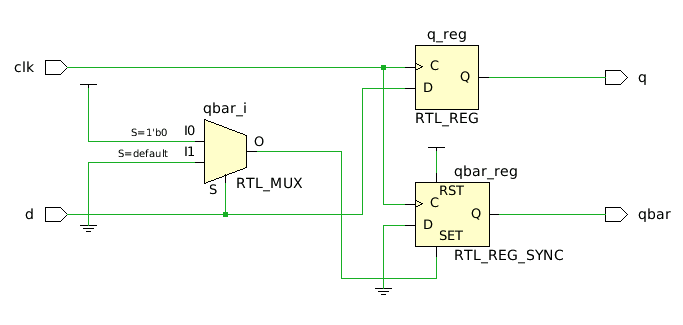
\includegraphics[width=0.65\textwidth]{DFlipFlop Schematic.png}
        \caption{D-Flip-Flop Schematic}
    \end{figure}
    \par This is the circuit created by the program for the D-flip-flop and once
    again, it is not the expected implementation for the flip-flop. As with the
    other experiments, the circuit must be simulated and the waveform must be
    analyzed to determine if the proper functionality is being attained.
    \begin{figure}[h]
        \centering
        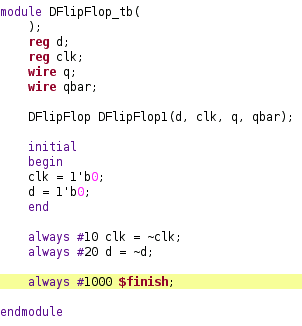
\includegraphics[width=0.4\textwidth]{DFlipFlop Simulation Code.png}
        \caption{D-Flip-Flop Simulation Code}
    \end{figure}
    \par In order to simulate this circuit the same procedure must be taken as
    with the other experiments in which the circuits were created using
    behavioral programming. In this case, as before, the inputs and outputs are
    initialized at the top of the module and the device in question is
    instantiated. Here, the "DFlipFlop" module is instantiated and given the
    inputs $d$ and $clk$ and outputs $q$ and $qbar$. Once that is done, the
    input values are defined as 00 and then a loop is created so that after a
    known time period, the value of the inputs change. In this case, every 10
    nanoseconds the value of $clk$ changes from its value to its compliment, and
    every 20 nanoseconds the value of $d$ changes to its compliment. The
    simulation is given a termination time of 1,000 nanoseconds and with that,
    the simulation is ready to be run.
    \begin{figure}[h]
        \centering
        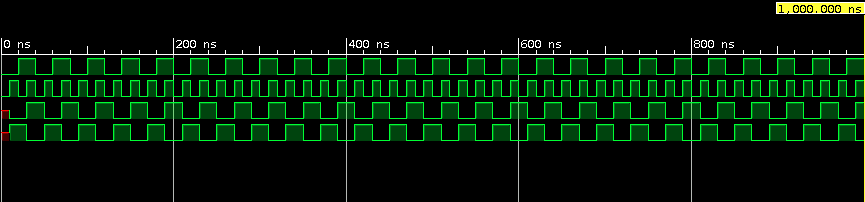
\includegraphics[width=1.0\textwidth]{DFilpFlop Waveform.png}
        \caption{D-Filp-Flop Waveform}
    \end{figure}
    \par This is the waveform generated for the D-flip-flop and the same
    analysis techniques must be employed to see if the circuit does indeed
    provide the correct functionality. Here, the top wave is that of the
    variable $d$, and the second is that of the clock, $clk$. The bottom two are
    $q$ and $qbar$ respectively once again. It can be seen here that at every
    positive edge of the clock, the output $q$ changes and no where else does it
    exhibit any change. This is the function of a flip-flop, the output will
    only change at the edge of the clock cycle. Looking further, it can be seen
    that the value of the output follows the current value of the input at the
    time of the positive edge cycle, when $d=1 \to q=1$ and when $d=0 \to q=0$,
    while the opposite is true for $qbar$. This is the exact function of the
    D-flip-flop as the inputs cause changes in the outputs however, the changes
    do not take affect until the positive edge of the clock cycle is reached.
    This elucidates that the generated circuit is indeed a D-flip-flop.
    \subsection*{Converting a D-Flip-Flop to a T-Flip-Flop}
    \begin{figure}[h]
        \centering
        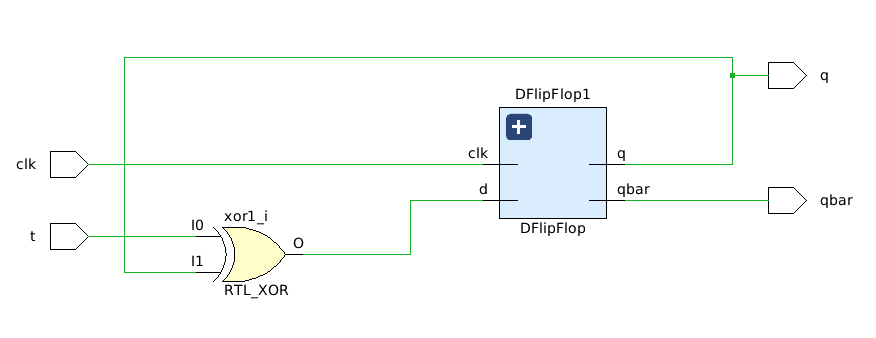
\includegraphics[width=0.9\textwidth]{TFlipFlop Schematic.png}
        \caption{T-Flip-Flop Schematic}
    \end{figure}
    \par When looking at a T-flip-flop, the main thing to notice is that the
    output is set to change at every full clock cycle. This differs from the
    operation of the D-flip-flop since that D-flip-flop changes at every
    positive edge of the clock cycle. With this generated schematic, it can be
    seen that the only alteration that needs to be made to the D-flip-flop is in
    the input variable $d$. Using an XOR gate, this can be achieved and the
    other inputs and outputs stay relatively the same.
    \begin{figure}[h]
        \centering
        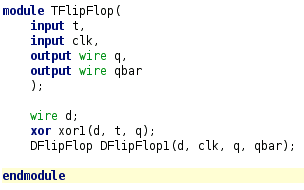
\includegraphics[width=0.4\textwidth]{TFlipFlop Code.png}
        \caption{T-Flip-Flop Code}
    \end{figure}
    \par This is the code for the implementation of the T-flip-flop and it is
    clear that there is only really one difference between the D and the T
    flip-flops since the T-flip-flop here can be seen to use the D-flip-flop
    module to attain functionality. The inputs here are $t$ and $clk$, and the
    outputs, $q$ and $qbar$, defined in the arguments of the module. The next
    aspect of this creation is the XOR gate and it takes in the values $t$ and
    $q$ and outputs to the wire $d$. Here, $d$ is defined as a wire and this
    wire is responsible for the connection of the XOR gate to the $d$ input of
    the D-flip-flop. Next comes the instantiation of the D-flip-flop module and
    it takes in the inputs, $d$ and $clk$, and output $q$ and $qbar$. Once
    again, to truly see the operation of the T-flip-flop we must look at the
    waveform generated by the circuit.
    \begin{figure}[h]
        \centering
        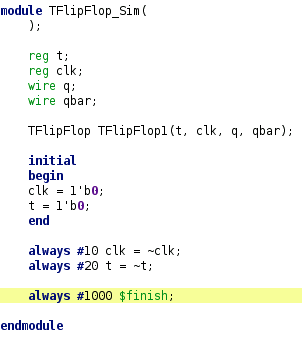
\includegraphics[width=0.4\textwidth]{TFlipFlop Simulation Code.png}
        \caption{T-Flip-Flop Simulation Code}
    \end{figure}
    \par This is the code for the simulation of the T-flip-flop circuit and it
    can be seen that it is in essence the same code as the simulation of the
    D-flip-flop, the only difference being that the T-flip-flop module is
    instantiated instead of the D-flip-flop. The inputs and outputs behave
    practically the same where $clk$ oscillates every 10 nanoseconds, and the
    input $t$ oscillates every 20 nanoseconds. The termination time is given
    once again at 1,000 nanoseconds.
    \begin{figure}[h]
        \centering
        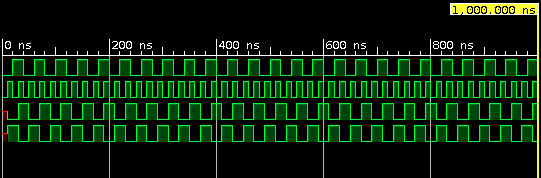
\includegraphics[width=1.0\textwidth]{TFlipFlop Waveform.png}
        \caption{T-Flip-Flop Waveform}
    \end{figure}
    \par Above is the waveform for what should be an operational T-flip-flop.
    This can be checked by simply analyzing where and how the outputs change
    within the waveform. The first wave at the top is the input $t$, the second
    is the clock $clk$, and the bottom two are the outputs $q$ and $qbar$. Now,
    simply by looking at the interval by which the output changes in relation to
    the clock, we can tell whether or not this is a T-flip-flop. It can be seen
    that the output changes every "wavelength" of the clock. This means that the
    output is changing after every one full cycle of the clock and since it can
    also be seen that the value of the output is in correspondence with the
    value of $t$, this device is providing the correct function of the
    T-flip-flop.
    \section*{Experiment 4}
    \begin{figure}[h]
        \centering
        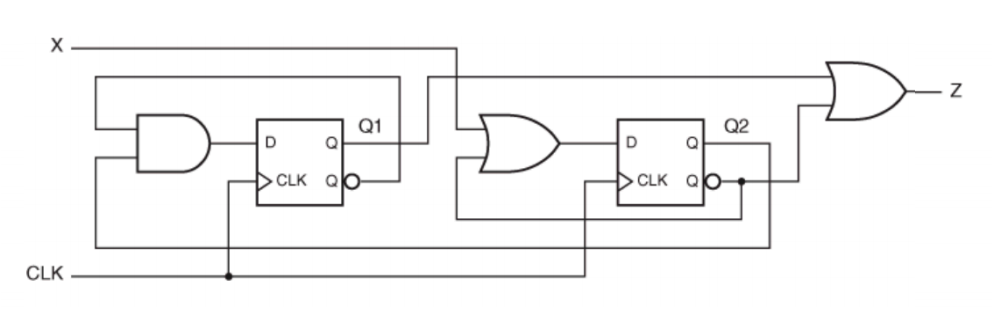
\includegraphics[width=0.85\textwidth]{Sequential Circuit Design.png}
        \caption{Sequential Circuit Design}
    \end{figure}
    \par Here is an example of a basic sequential circuit, it uses two
    flip-flops along with combinational gates to take an input and a clock, and
    form an output. Since it contains two D-flip-flops, there will be a possible
    4 states in which the circuit can reside. We will first analyze this state
    machine and then work to implement it using Verilog in order to observe its
    waveform.
    \par The first step in the analysis of a state machine is the determination
    of whether the machine is a Mealy or a Moore machine. In this case, the
    circuit can be seen to have one input variable, $x$, and this variable is
    seen to have no direct connection to the output variable $z$. For this
    reason, this is a Moore state machine.
    \par Next comes the definition of the excitation equations and since we have
    two flip-flops, we will name the inputs $D_1$ and $D_2$. It can be seen that
    the input $D_1$ is the output of an AND gate and looking at the inputs of
    the AND gate we can see that the expression for $D_1$ will be $Q_1' Q_2$.
    For the second equation, the input $D_2$ is the output of an OR gate, and
    the inputs of this OR gate are $x$ and $Q_2'$. This leaves the expression
    for $D_2$ to be $x+Q_2'$.
    \par The next step is the creation and analysis of the characteristic
    equation for the flip-flops within the circuit. Since the only flip-flop in
    use here is the D-flip-flop, the characteristic equations are given as $Q_1*
    = D_1$ and $Q_2* = D_2$, where $Q_1*$ and $Q_2*$ represent the next state of
    the flip-flop. Once these are defined, the expressions can be substituted in
    yielding the transition equations, $Q_1* = Q_1' Q_2$ and $Q_2* = x + Q_2'$.
    \par Now that the transition equations have been attained, the transition
    table for this circuit can be formed.
    \begin{table}[h]
        \centering
        \begin{tabular}{cc|cc}
            \toprule
            $Q_1$ & $Q_2$ & $x=0$ & $x=1$ \\
            \midrule
            0 & 0 & 01 & 01 \\
            0 & 1 & 10 & 11 \\
            1 & 0 & 01 & 01 \\
            1 & 1 & 00 & 01 \\
            \bottomrule
        \end{tabular}
        \caption{Transition Table}
    \end{table}
    \par This is the transition table for the given circuit. The right hand side
    of the table gives the values of $Q_1*$ and $Q_2*$ and those values are
    derived straight from the transition equations. Now that we have the
    transition table, the state and state/output tables can be derived. For the
    state/output table, the output equation is required. This equation can be
    granted straight from the analysis of the circuit, just as the excitation
    equations were determined. It can be seen that the output variable $z$ is
    the result of an OR gate and the inputs to this OR gate can be traced back
    to $Q_1$ and $Q_2'$. This gives the output equation $z = Q_1 + Q_2'$.
    \par Now that we have the transition table as well as the output equation,
    the states must be defined and from there the state/output table can be
    constructed. The states can simply be defined as the value of $Q_1 Q_2$, 00,
    01, 10, and 11:
    \begin{table}[h]
        \centering
        \begin{tabular}{c|cc}
            States & $Q_1$ & $Q_2$ \\
            \midrule
            A & 0 & 0 \\
            B & 0 & 1 \\
            C & 1 & 0 \\
            D & 1 & 1 \\
        \end{tabular}
    \end{table}
    \par With these states, the state/output table can be constructed and simply
    requires the substitution of the individual states within the transition
    table, as well as the definition of the output based on its equation.
    \begin{table}[h]
        \centering
        \begin{tabular}{c|cc|c}
            \toprule
            $S$ & $x=0$ & $x=1$ & $z$ \\
            \midrule
            A & B & B & 1 \\
            B & C & D & 0 \\
            C & B & B & 1 \\
            D & A & B & 1 \\
            \bottomrule
        \end{tabular}
        \caption{State/Output Table}
    \end{table}
    \par This is the state/output table for the circuit and describes the
    transitions between the different states of the machine, as well as the
    outputs of the machine with each given transition. Now, this design must be
    implemented using Verilog which will allow for the generation of the
    waveform of the circuit.
    \newpage
    \begin{figure}[h]
        \centering
        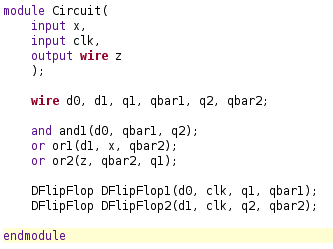
\includegraphics[width=0.35\textwidth]{Sequential Circuit Code.png}
        \caption{Sequential Circuit Code}
    \end{figure}
    \par This is the code for the implementation of the circuit. From the design
    it can be seen that it uses some basic gates as well as two D-flip-flops and
    in the code, exactly what is needed to create the circuit. Since there are
    two inputs and one of them is the clock, there is really only one input that
    needs to be monitored in the end. The inputs are defined as $x$ and $clk$,
    and the output is given as a wire, $z$. Next, there are multiple additional
    wires that are defined and these are responsible for the connections between
    each of the gates and the flip-flops. The wires $d 0$ and $d 1$ are the
    inputs to the flip-flops and $q 1$, $q 2$, and $qbar 1$, $qbar 2$, are the
    outputs of the flip-flops.
    \par Now for the basic gates, one AND gate and two OR gates are defined
    corresponding to the ones seen in the design. The AND gate will take the
    inputs $qbar 1$ and $q 2$ and output through the wire $d 0$, the input of
    the first flip-flop. Next come the OR gates, the first one corresponding to
    the input of the second flip-flop and the second corresponding to the
    formation of the output. The first OR gate takes the inputs $x$ and $qbar 2$
    and outputs $d 1$, the input of the second flip-flop, and the second OR gate
    takes the inputs $qbar 2$ and $q 1$, and gives the output $z$.
    \par Lastly, the flip-flops themselves have to be defined. This is done by
    using the previous module that was created. The two flip-flops will each
    take in one of the two outputs of the AND and the OR gates, $d 0$ and $d 1$,
    as well as the clock $clk$. The outputs to each of the flip-flops are given
    as the respective $q$ and $qbar$. Now that the module for the circuit is
    created, the schematic can be generated and the simulation can be
    constructed.
    \begin{figure}[h]
        \centering
        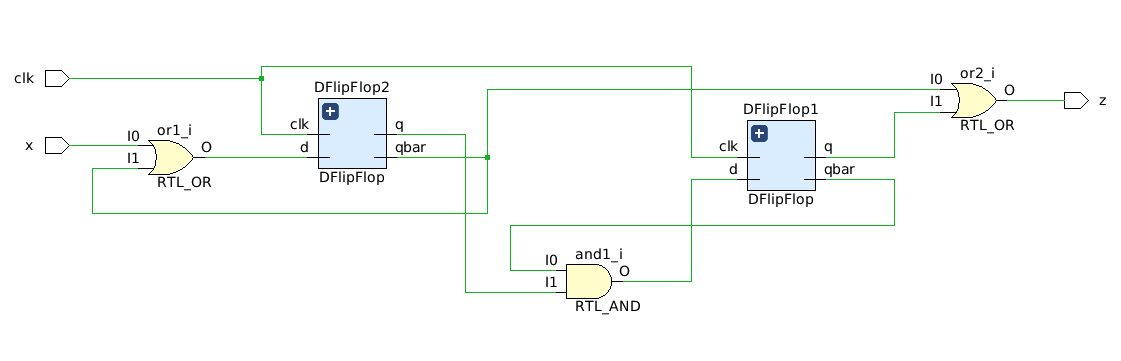
\includegraphics[width=0.9\textwidth]{Sequential Circuit Schematic.png}
        \caption{Sequential Circuit Schematic}
    \end{figure}
    \begin{figure}[h]
        \centering
        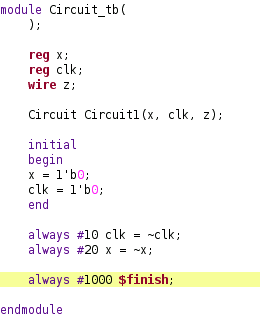
\includegraphics[width=0.3\textwidth]{Sequential Circuit Simulation Code.png}
        \caption{Sequential Circuit Simulation Code}
    \end{figure}
    \par The code above is for the test bench and the simulation of the circuit.
    This code follows the same principles as the previous simulation. At the
    top, the inputs, $x$ and $clk$, and the output, $z$, are initialized and the
    circuit itself is instantiated with the inputs and the output. After this,
    the simulation is began and the inputs are given values of 00. Now that the
    initial values are set, every 10 nanoseconds the clock is set to oscillate
    and every 20 nanoseconds as does the value of $x$. The simulation is given a
    termination time of 1,000 nanoseconds and with that, the waveform is ready
    to be generated.
    \begin{figure}[h]
        \centering
        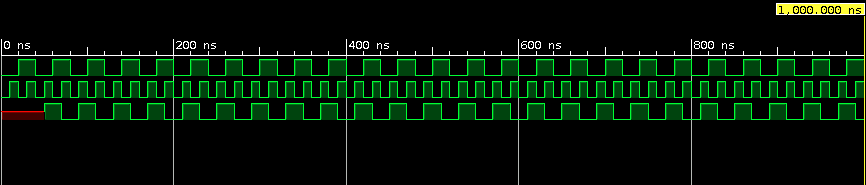
\includegraphics[width=1.0\textwidth]{Sequential Circuit Waveform.png}
        \caption{Sequential Circuit Waveform}
    \end{figure}
    \par This is the waveform that is generated by the circuit and the first
    thing to notice is that the output changes on the positive edge of the
    clock. This is expected behavior since we deduced that this was a Moore
    Machine, a machine whose output changes at the edge of the clock and not
    upon the instant alteration of the input. The first wave is that of the
    variable $x$, the second of the clock, and the last of the output $z$. It
    can be seen that $z$ changes in accordance to the equations that were
    defined previously and for this reason, it can be confirmed that the
    equations created and the state/output table formed for this machine was in
    fact the correct progression of states.
\end{document}
